%\subsection{Simplicial Complexes}
\textbf{Simplicial Complexes.} A \emph{simplicial complex} is a collection of finite sets closed under taking subsets. We refer to a set in a simplicial complex as a \emph{simplex} of \emph{dimension $p$} if it has cardinality $p+1$. Such a $p$-simplex has $p+1$ \emph{faces} of dimension $p-1$, namely the sets omitting one element, which we will denote as $[v_0,\dotsc,\hat{v}_i,\dotsc, v_p]$ when omitting the $i$'th element. While this definition is entirely combinatorial, there is a geometric interpretation, and it will make sense to refer to and think of $0$-simplices as \emph{vertices}, $1$-simplices as \emph{edges}, $2$-simplices as \emph{triangles}, $3$-simplices as \emph{tetrahedra}, and so forth (see Figure~\ref{fig:data2complex}, (b)). Let $C_p(K)$ be the free real vector space with basis $K_p$, the set of $p$-simplices in 
a simplicial complex $K$. The elements of $C_p(K)$ are called \emph{$p$-chains}. The 
$p$-cochain (vector) space $C^p(K)$ is defined as the dual of $C_p(K)$, i.e. $C^p(K)=\hom(K_p,\RR)$. These vector spaces come equipped with \emph{coboundary maps}, namely linear maps $\delta^p:C^p\to C^{p+1}$ defined by
\begin{equation*}
\delta^p(f)([v_0,\dotsc,v_{p+1}]) = \sum_{i=0}^{p+1} (-1)^i f([v_0,\dotsc,\hat{v}_i,\dotsc,v_{p+1}]).
\end{equation*}
\begin{figure}[htpb]
%\begin{table*}[!t]
\savebox{\tempbox}{% compute size of tabulat
\scriptsize{
\begin{tabular}{llll}
    \cmidrule(r){1-3}
    Papers   & Authors     & Citations  \\
    \midrule
    Paper I & A, B, C  & 100  \\
    Paper II &  A, B & 50\\ 
    Paper III & A, D & 10\\ 
    Paper IV & C, D & 4\\ 
    \bottomrule
  \end{tabular}
}}%
\settowidth{\tempwidth}{\usebox{\tempbox}}%
\hfil\begin{minipage}[b]{\tempwidth}%
\raisebox{-\height}{\usebox{\tempbox}}%
%\vspace{-7pt}
\scriptsize{\caption*{(a)}}%
\label{table:data}%
\end{minipage}%
\savebox{\tempbox}{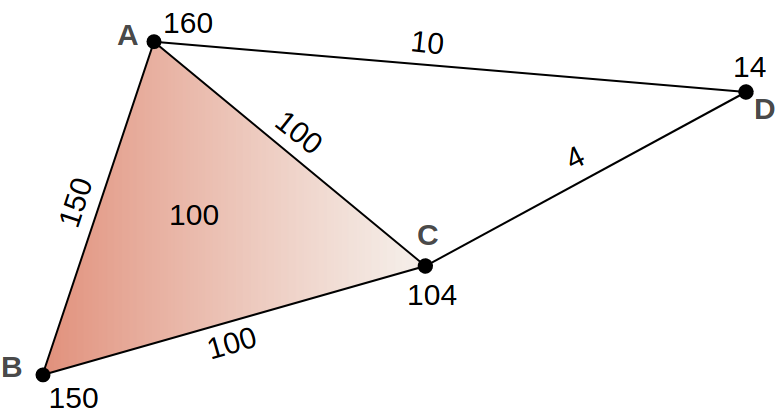
\includegraphics[height=2.3cm]{./figures/cc1.png}}%
\settowidth{\tempwidth}{\usebox{\tempbox}}%
\hfil\begin{minipage}[b]{\tempwidth}%
\raisebox{-\height}{\usebox{\tempbox}}%
\scriptsize{\captionof*{figure}{(b)}}%
\label{fig:co-authoship-complex}%
\end{minipage}%
\vspace{5pt}
%\end{table*}
\savebox{\tempbox}{\scriptsize{
\begin{blockarray}{cccccc}
\tiny{AB} & \tiny{AC} & \tiny{AD} & \tiny{BC} & \tiny{CD} \\
\begin{block}{(ccccc)c}
  3 & 0 & 1 & 0 & 0 & \tiny{AB} \\
  0 & 3 & 1 & 0 & -1 & \tiny{AC} \\
  1 & 1 & 2 & 0 & 1 & \tiny{AD} \\
  0 & 0 & 0 & 3 & -1 & \tiny{BC}\\
  0 & -1 & 1 & -1 & 2 & \tiny{CD}\\
\end{block}
\end{blockarray}}}%
\settowidth{\tempwidth}{\usebox{\tempbox}}%
\hfil\begin{minipage}[b]{\tempwidth}%
\raisebox{-\height}{\usebox{\tempbox}}%
\scriptsize{\captionof*{figure}{(c)}}%
\end{minipage}%
%\end{table*}
\caption{Example of co-authorship complex and its $1$-Laplacian. (a) Data. (b) Co-authorship complex with corresponding cochains build from the data. (c) $1$-Laplacian associated to the co-authorship complex. }\label{fig:data2complex}
\end{figure}

%\subsection{Simplicial Laplacians}
\textbf{Simplicial Laplacians.} We are in this paper concerned with finite abstract simplicial complexes. Albeit our method is applicable to a larger set of topological spaces, such as finite CW-complexes, where one has a notion of finite cochains. 
%In particular, it is not necessary for the simplicial complexes to come equipped with some embedding into Euclidean spaces, nor do we demand that they triangulate a Riemannian manifold.
To define a discrete version of the Laplacian for simplicial complexes, one simply takes the linear adjoint of the coboundary operator with respect to the inner product, defining $\delta_i^\ast:C^{i+1}\to C^i$ by
\begin{equation*}
  \ip{\delta_i f_1}{f_2}_{i+1} =\ip{f_1}{\delta_i^\ast f_2}_{i},\ \forall f_1\in C^{i}(K), f_2 \in C^{i+1}(K).
\end{equation*}

In analogy with Hodge--de Rham theory~\cite{madsen1997calculus}, we then define the \emph{degree-$i$ simplicial Laplacian} of a simplicial complex $K$ as the linear operator $\lap_i:C^i(K)\to C^i(K)$ such that
\begin{equation*}
  \lap_i = \lapu_i + \lapd_i,\\
\end{equation*}
where $\lapu_i =  \delta_{i}^\ast\circ\delta_{i}$ and $\lapd_i = \delta_{i-1}\circ\delta_{i-1}^\ast$. In case $i=0$, $\mathcal{L}_0$ corresponds to the classical graph Laplacian. Observe that there are $p$ Laplacians for a complex of dimension $p$. \stefania{What about moving the following paragraph in the supplementary?}In most practical applications, the matrices for the Laplacians are very sparse and can easily be computed as a product of sparse coboundary matrices and their transposes. Since the Laplacians encode information about the adjacency of the simplices, they can be interpreted as a message passing functions~\cite{gilmer2017NeuralMP}. Additionally, they carry valuable topological information about the simplicial complex. In particular, the kernel of the $k$-Laplacian is isomorphic to the $k$-(co)homology of its associated simplicial complex ~\cite{eckmann1944,horak2013spectra}.
% In other words, the number of zero-eigenvalues tells us the number of $k$-dimensional holes~\cite{horak2013spectra}.
